\section{Jan Banasik}
\label{sec: jbanasik}

Zacznijmy od czegoś prostego, a więc od Całki Gaussa:
\[ \int_{-\infty}^{\infty}\ e^{-x^2} dx = \sqrt{\pi} \]
To może teraz jedynka trygonometryczna: \[ sin^{2}(\alpha) + \cos^{2}(\alpha)= 1 \]

\begin{figure}[h!]
    \centering
    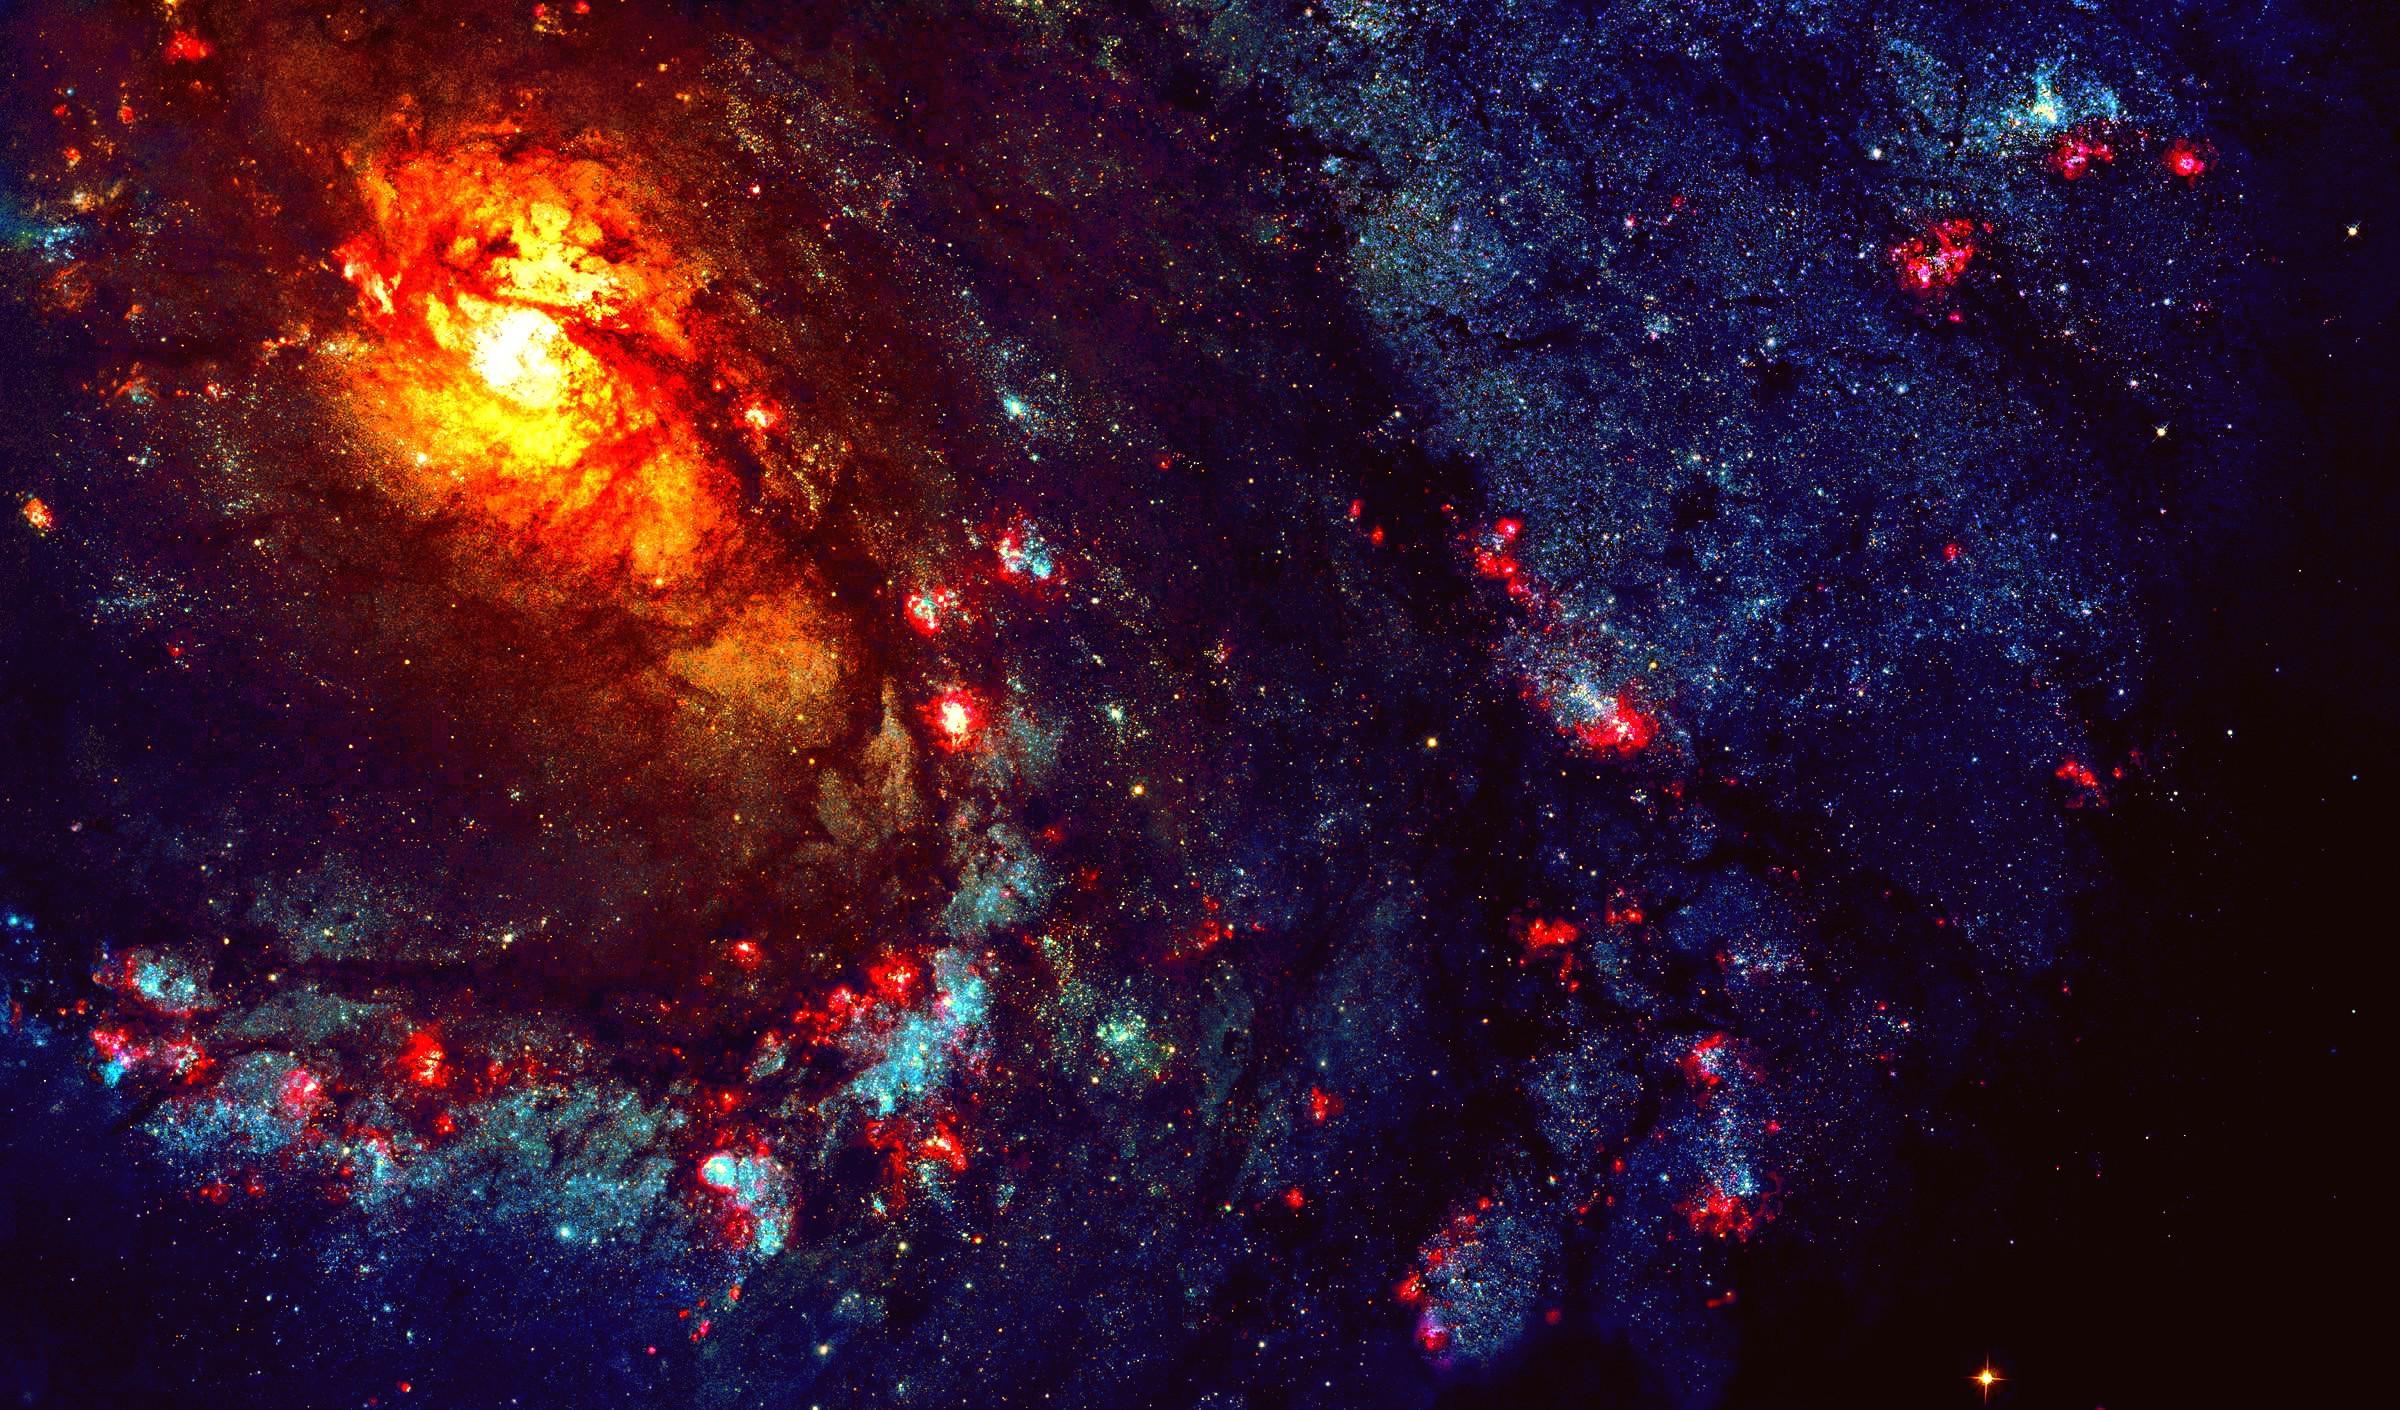
\includegraphics[width = 0.9\textwidth]{pictures/galaxy.jpg}
    \caption{Galaxy}
    \label{fig:galaxy}
\end{figure}

Look at that Figure \ref{fig:galaxy} that's pretty, isn't it? 

\begin{table}[h]
\centering
\begin{tabular}{|l|l|l|l|}
\hline
\textbf{n}          & \textbf{n!}           & \textbf{n**2}        & \textbf{sqrt(n)}       \\ \hline
\textbf{0}          & \textbf{1}            & \textbf{0}           & \textbf{0.00}             \\ \hline
\textbf{1}          & \textbf{1}            & \textbf{1}           & \textbf{1.00}             \\ \hline
\textbf{2}          & \textbf{2}            & \textbf{4}           & \textbf{1.41}          \\ \hline
\textit{\textbf{3}} & \textit{\textbf{6}}   & \textit{\textbf{9}}  & \textit{\textbf{1.73}} \\ \hline
\textit{\textbf{4}} & \textit{\textbf{24}}  & \textit{\textbf{16}} & \textit{\textbf{2.00}} \\ \hline
\textit{\textbf{5}} & \textit{\textbf{120}} & \textit{\textbf{25}} & \textit{\textbf{2.23}} \\ \hline
\end{tabular}
\label{tab: functions}
\caption{Podstawowe funkcje matematyczne}
\end{table}


Tabela \ref{tab: functions} przedstawia podstawowowe funkcje matematyczne 
\newpage

\href{https://www.chess.com/players}{\textbf{TOP 5 BEST CHESS PLAYERS IN THE WORLD}} \footnote{Ranking może ulec zmianie na przestrzeni czasu, dane są podane na dzień 26.10.2023}
\begin{enumerate}
    \item  \textbf{Magnus Carlsen}
    \item  \textit{Fabiano Caruana}
    \item  \underline{Ding Liren}
    \item  \textbf{Hikaru Nakamura}
    \item  \textit{Alireza Firouzja} \newline\newline
\end{enumerate}



\textbf{Nie zapominajmy o naszych wspaniałych, wybitnych polskich pisarzach:}
\begin{itemize}
    \item[!] \emph{Henryk Sienkiewicz}
    \item[@] \textsc{Adam Mickiewicz}
    \item[?] \emph{Juliusz Słowacki}
    \item[/] \textsc{Stanisław Lem} \\
\end{itemize}

A na koniec trochę poezji:


\begin{center}
    \textbf{Inwokacja}
\end{center}

\textbf{LITWO, OJCZYZNO MOJA!} \\
Litwo, Ojczyzno moja! ty jesteś jak zdrowie; \\
Ile cię trzeba cenić, ten tylko się dowie, \\
Kto cię stracił. Dziś piękność twą w całej ozdobie \\
Widzę i opisuję, bo tęsknię po tobie. 

Panno święta, co Jasnej bronisz Częstochowy \\
I w Ostrej świecisz Bramie! Ty, co gród zamkowy\\
\textsc{Nowogródzki ochraniasz z jego wiernym ludem!\\
Jak mnie dziecko do zdrowia powróciłaś cudem\\
(— Gdy od płaczącej matki, pod Twoją opiekę\\
Ofiarowany martwą podniosłem powiekę;\\
I zaraz mogłem \underline{pieszo}, do Twych świątyń progu\\
Iść za wrócone życie podziękować Bogu —)}\\
Tak nas powrócisz cudem na Ojczyzny łono!...\\
Tymczasem, przenoś moją \emph{duszę utęsknioną}\\
\textbf{Do tych pagórków leśnych, do tych łąk zielonych,\\
Szeroko nad błękitnym Niemnem rozciągnionych;\\
Do tych pól malowanych zbożem rozmaitem,}\\
\textbf{\textit{Wyzłacanych pszenicą, posrebrzanych żytem;}}\\
Gdzie bursztynowy świerzop, gryka jak śnieg biała,\\
Gdzie panieńskim rumieńcem dzięcielina pała,\\
A wszystko przepasane jakby wstęgą, miedzą\\
Zieloną, na niej zrzadka ciche grusze siedzą.\\
















